% !TeX encoding = UTF-8
% !TeX program = xelatex
% !TeX spellcheck = en_US

\documentclass[a4paper]{article}
\usepackage{amsmath}
\usepackage[english]{babel}
\usepackage[UTF8]{ctex}
\usepackage{unicode-math}
\usepackage{caption}
\usepackage{booktabs}
\usepackage{xcolor}
\usepackage{array}
\usepackage{listings}
\usepackage{hypdoc}
\usepackage[left=0.50in,right=0.50in,top=1.0in,bottom=1.0in,paperheight=11in,paperwidth=8.5in]{geometry}
\usepackage{endnotes}
\usepackage{graphicx}
\usepackage{multicol}
\usepackage{float}
\usepackage{blindtext}
\usepackage{listings}
\usepackage{xcolor}

\title{Lab report:\\Experimenting with digital meter assembly}
\author{Tiankai Ma PB21000030}
\date{\today}
\begin{document}
\begin{multicols*}{2}
    \maketitle
    \begin{abstract}
        Digital meter plays a more and more important role in electrical experiments, understanding how it works helps improve experiment design and reduce the risk of accidents. This report will introduce the working principle of the digital meter and the assembly of the digital meter and gives a brief description of how its impact on the measuring system.
        \par
        \textbf{Keywords:} Digital meter, Electrical experiments, Measuring system
    \end{abstract}
    \section*{Introduction}

    \subsection*{Digital meter}

    Compared to the analog meter, the digital meter has more advantages. It is more accurate, more stable, and more convenient to use. In this experiment, we are going to expand its features to adapt it for voltage, current, and resistance measurement. More importantly, by experimenting with how measuring equipment impacts measured results, we will learn how to design a better measuring system.

    \textbf{Features of digital meter:}

    Compared to pointer meters, digital meters have the following excellent characteristics.

    \begin{itemize}
        \item High accuracy and resolution
        \item Digital voltmeter has a high input impedance
        \item Fast measurement rate
        \item Automatic polarity discrimination
        \item Digital direct reading of all measurements
        \item High overload resistance
    \end{itemize}

    \subsection*{DC Voltage Measurement Circuit}

    The range of DC voltage measurement can be extended by adding a voltage divider circuit(voltage divider)in front of the digital voltmeter head. As shown in Figure 1, $U_0$ is the range of the digital voltmeter head (e.g. $200mV$), $r$ is its internal resistance (e.g. $10MΩ$), $r_1$ and $r_2$ are the voltage divider resistors, and Ui0 is the extended range.

    \begin{figure}[H]
        \centering
        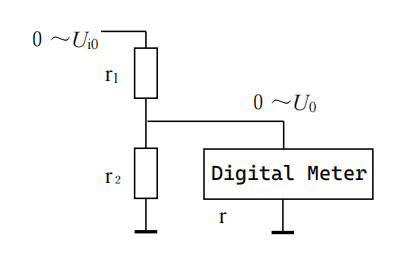
\includegraphics[width=0.8\linewidth]{./img/Fig.1.png}
        \caption{Single range voltage divider circuit}
        \label{fig:figure1}
    \end{figure}

    If we have $r >> r_2$, the impact of r could be ignored, we have the following equation:

    $$
        \dfrac{U_0}{U_{i0}} = \dfrac{r_2}{r_1 + r_2}
    $$

    The extended range is $U_{i0} = U_0 \cdot \dfrac{r_1 + r_2}{r_2}$.

    \subsection*{Analysis of the measurement error}

    During measurement, the error comes mainly from two aspects: one is introducing the meter inside the circuit, which stays the same throughout the measurement, the is considered a system error; the other is caused by the assembled meter, which is considered a random error.

    \textbf{System error:}

    Since the internal resistance of the voltmeter is not infinite, using a voltmeter to measure the voltage across the circuit components will affect the measurement results. We use the measurement circuit shown in Figure 2 to analyze the measurement error of the assembled meter and accordingly study the effect of the measuring instrument on the measurement results.


    \begin{figure}[H]
        \centering
        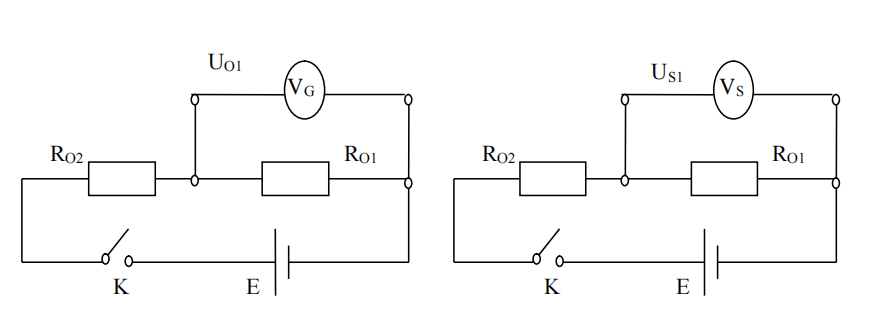
\includegraphics[width=0.8\linewidth]{./img/Fig.2.png}
        \caption{Comparison of the measurement error of the assembled meter}
        \label{fig:figure2}
    \end{figure}

    The measured data should be expressed in the following equation:

    \begin{equation}
        \left\{
        \begin{aligned}
            U_{s1} & = E \cdot \dfrac {R_{o1}} {R_{o1} + R_{o2}}                             \\
            U_{o1} & = E \cdot \dfrac {R_{o1} \mid\mid R_g} {(R_{o1} \mid\mid R_g) + R_{o2}} \\
        \end{aligned}
        \right.
    \end{equation}

    Where $R_{o1} \mid\mid R_g = \dfrac{R_{o1} \cdot R_g}{R_{o1} + R_g}$.

    The relative error caused by the meter could then be expressed as:

    $$
        \dfrac{U_{s1} - U_{o1}}{U_{s1}} = \dfrac{R_{o2}}{R_{o1} + R_{o2}} \cdot \dfrac{R_{o1} \mid\mid R_g}{R_{o1} \mid\mid R_g + R_{o2}} = \dfrac{1} {1 + \dfrac{R_{g}}{R_{o1} \mid\mid R_g}}
    $$

    Based on the analysis above, it can be seen that the error caused by the meter is related not only to $R_g$, but also to $R_{o1} \mid\mid R_{o2}$. The larger the value of $\dfrac{R_g}{R_{o1} \mid\mid R_{o2}}$ is, the smaller the error caused by the meter is.


    \textbf{Random error:}

    The uncertainty of the measurement results could be calculated with the following equation:

    \begin{equation}
        \begin{split}
            u_{U_0} = \left[\left(\dfrac{r_2}{r_1 + r_2} \cdot u_{U_{i0}}\right)^2 + \right.\\\left.\left(\dfrac{r_1}{(r_1 + r_2)^2} \cdot u_{r_{2}}\right)^2 + \left(\dfrac{r_2}{(r_1 + r_2)^2} \cdot u_{r_{1}}\right)^2 \right]^{1/2}
        \end{split}
    \end{equation}

    To correct random error, a calibration curve is recommended to compensate the error.

    \section*{Materials}

    \subsection*{Instrument check}

    skipped.

    \subsection*{Design a multi-range DC voltmeter}

    Requirements: design and construct a multi-range DC voltmeter with a range of $0-200mV$, $0-2V$, $0-20V$, $0-200V$ and $0-1000V$, show related $R_1, R_2$ values, and the corresponding measurement range.

    \subsection*{Error analysis}

    Requirements: analyze the difference between the measurement results of the assembled meter and the a given voltmeter, and calculate the error caused by the meter.

    \subsection*{Calibration curve}

    Requirements: record a calibration curve for the assembled meter, and use it to correct the random error.

    \section*{Results}

    \subsection*{Design a multi-range DC voltmeter}

    \begin{tabular}{l|l|l|l|l|l}
        range & $200mv$      & $2v$        & $20v$       & $200v$        & $2000v$        \\ \hline
        $R_1$ & $100k\Omega$ & $10k\Omega$ & $1k\Omega$  & $0.1k\Omega$  & $0.01k\Omega$  \\
        $R_2$ & $0k\Omega$   & $90k\Omega$ & $99k\Omega$ & $99.9k\Omega$ & $99.99k\Omega$
    \end{tabular}

    \begin{figure}[H]
        \centering
        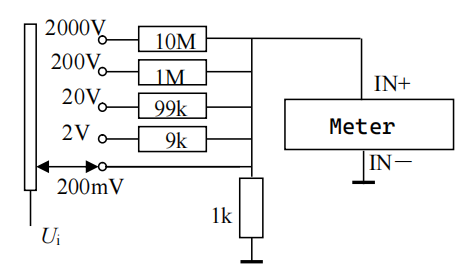
\includegraphics[width=0.8\linewidth]{./img/Fig.3.png}
        \caption{Multi-range DC voltmeter}
        \label{fig:figure3}
    \end{figure}

    The circuit is shown as Figure.3, the max range is $100k\Omega * 0.07A = 7kV$

    \subsection*{Error analysis}

    $R_1 = 10k\Omega, R_2 = 90k\Omega, R_g = 100k\Omega, U=5V$

    The results are shown as:

    \begin{tabular}{l|l|l|l|l}
        $R_{o1}=R_{o2}(\Omega)$ & 100   & 500   & 1k    & 5k    \\\hline
        $U_{s1}(V)$             & 2.522 & 2.526 & 2.524 & 2.524 \\
        $U_{o1}(V)$             & 2.517 & 2.514 & 2.510 & 2.458 \\\hline
        $R_{o1}=R_{o2}(\Omega)$ & 10k   & 20k   & 40k   & 60k   \\\hline
        $U_{s1}(V)$             & 2.521 & 2.522 & 2.517 & 2.514 \\
        $U_{o1}(V)$             & 2.399 & 2.289 & 2.100 & 1.937 \\\hline
        $R_{o1}=R_{o2}(\Omega)$ & 80k   & 100k  & 1M    & 2M    \\\hline
        $U_{s1}(V)$             & 2.512 & 2.509 & 2.444 & 2.310 \\
        $U_{o1}(V)$             & 1.798 & 1.679 & 0.422 & 0.229 \\
    \end{tabular}

    \subsection*{Calibration curve}

    \begin{tabular}{l|l|l|l|l|l|l|l|l|l|l|l}
        $R_{o1}$ & 0   & 20     & 40     & 60     & 80     & 100    & 120    & 140    & 160    & 180    & 200    \\\hline
        $R_{o2}$ & 500 & 480    & 460    & 440    & 420    & 400    & 380    & 360    & 340    & 320    & 300    \\\hline
        $U_{s1}$ & 0   & 0.2032 & 0.4062 & 0.6093 & 0.8122 & 1.0151 & 1.2170 & 1.4197 & 1.6227 & 1.8254 & 1.9269 \\
        $U_{o1}$ & 0   & 0.2011 & 0.4023 & 0.6036 & 0.8047 & 1.0057 & 1.2057 & 1.4066 & 1.6077 & 1.8087 & 1.9093
    \end{tabular}

    \par*
    \textbf{Images are shown in seprate page.}
    \columnbreak

    \section*{References}
    \textit{Most contents were translated from the handout.}

    \section*{Acknowledgements}
    This is the last experiment of this course, and perhaps the last physics experiment I'll ever have in USTC. There was time I really hate this course, as most of the experiments were boring and just meaningless repeats, but by the end of this course, I really enjoy the experiments and learned a lot from it, I learned how to use latex, how to use python, I learned how to analyze data and make beautiful charts.

    I would take this chance to thank all the teachers and TAs for your amazing job, and for those who offered help and encouragement, my sincere and hearty thanks and appreciations goes to all of you.
    \newpage
\end{multicols*}
\section*{Images}
\begin{figure}[H]
    \centering
    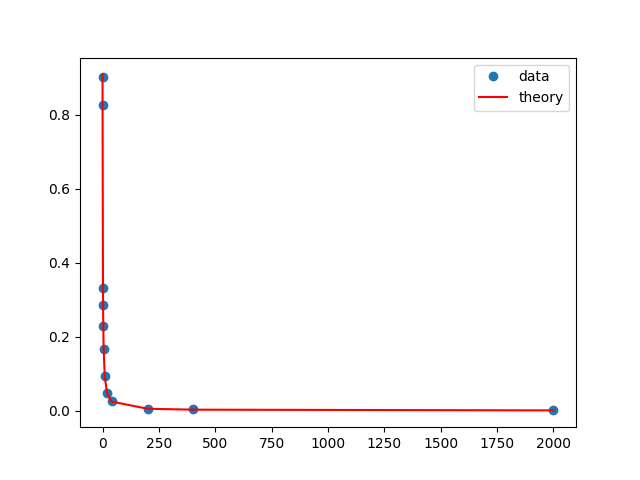
\includegraphics[width=0.6\linewidth]{./img/Fig.4.png}
    \caption{Error analysis}
\end{figure}
\begin{figure}[H]
    \centering
    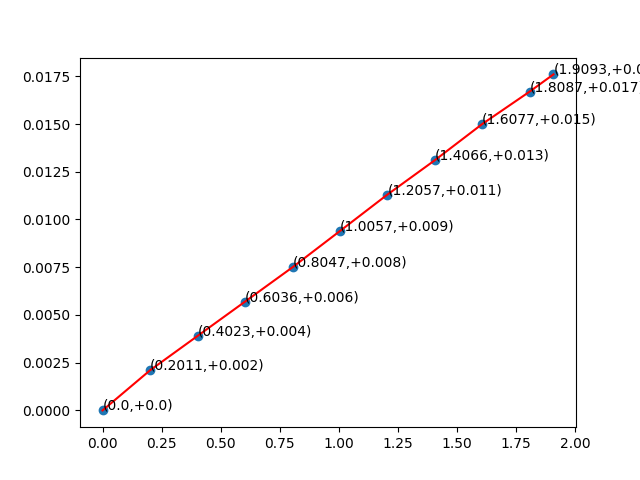
\includegraphics[width=0.6\linewidth]{./img/Fig.5.png}
    \caption{Calibration curve}
\end{figure}
\end{document}